\chapter{Contributions}
\section{Submodules and Specifications}
%%talk about the specs


The main focus of this thesis will be on 2 important submodules in charge of their load instructions:\\

\textit{Load Buffer} and \textit{Load Management Unit}.

\subsection{Load Management Unit}
%general


This module is in charge of handling the load operations.
Those can be strided or indexed.\\

Since the VPU is able to work out-of-order an ID system is necessary, so each instructions comes with an ID.
In particular the load operation come with the signal \textbf{seq\+id\+i}.
This signal contains all the informations about the issued load.\\

The main elements of this submodules are:
\begin{itemize}
    \item \textit{Shifter}: it is useful to have the first bit not in the MSB or LSB position.
    
    \item \textit{Compactor}: it is useful to compact all the valid elements. When the stride = 1 there is no use of the compactor.
    
    \item \textit{Aligner}: it is in charge to align the elements for the output (lane, bank and sub-bank).
\end{itemize}

\bigskip

%params
The main parameters defining this submodule are:
\begin{itemize}
    \item \textbf{MEM\+DATA\+WIDTH}: width of the chunk of data received from Avispado. The standard value is \textit{512}.
    
    \item \textbf{SEQ\+ID\+WIDTH}: width of the \textit{seq\+id\+i} that identifies the data coming from Avispado. The standard value is \textit{33}.
    
    \item \textbf{MAX\+NUMBER\+ELEMENTS}: maximum number of elements that can be encoded in the chunk of data received (64 when SEW = 8 bit). The standard value is \textit{64}.
    
    \item \textbf{MAVISPADO\+LOAD\+MASK\+WIDTH}: Indicates the maximum number of mask bits that are received with the data. Every bit of the mask represent a byte into the data. The standard value is \textit{64}.
    
    \item \textbf{NUM\+LANES}: number of lanes. The standard value is \textit{8}.
\end{itemize}

\subsubsection{Interface}
%interface
%%%%%%%%%%%%%%%%TABLE%%%%%%%%%%%%%%%%%%%%%%%

\begin{table}[H]
\centering
\begin{tabular}{|l|l|}
\hline
\rowcolor[HTML]{EFEFEF} 
\multicolumn{1}{|c|}{\cellcolor[HTML]{EFEFEF}Signal} & \multicolumn{1}{c|}{\cellcolor[HTML]{EFEFEF}Description}                      \\ \hline
load\+granted\+i    & a load is granted,\\
                    & it will have a certain sew\+i and stride\+i\\ \hline
load\+granted\+sb\+id\+i    & the id for the issued Load,\\
                            & can be issued up to 2 loads\\ \hline
indexed\+load\+granted\+i   & the granted load is indexed \\ \hline
load\+data\+valid\+i        & indicates if the data in load\+data\+i bus is valid\\ \hline
load\+data\+i               & data received from Avispado\\ \hline
seq\+id\+i                  & the sequence id (described below)\\ \hline
mask\+valid\+i              & validity of mask\+i signal\\ \hline
mask\+i                     & mask bits to mask load\+data\+i\\ \hline
sew\+i                      & identifies the size of each vector element\\ \hline
stride\+i                   & stride indicated in bytes\\ \hline
load\+data\+o               & output data sent to the lanes\\ \hline
load\+dvalid\+o             & indicates if the data in load\+data\+o bus is valid\\ \hline
mask\+o                     & mask bits to mask load\+data\+o\\
                            & it is needed also for not masked inst.\\ \hline
element\+ids\+o             & identifies each element sent in load\+data\+o\\ \hline
sb\+id\+o                   & identifies the instruction\\ \hline
vstart\+self\+o             & identifies the first valid element\\
                            & in the chunk of data received in load\+data\+i\\ \hline
vstart\+next\+o             & identifies the last valid element \\
                            & in the chunk of data received in load\+data\+i\\ \hline
min\+element\+id\+idx\+o    & index of the first valid \\
                            & element in elements\+ids\+o of each lane.\\ \hline
\end{tabular}
\end{table}


\subsubsection{Sequence ID}
The sequence id ID is very useful as the memory system does not guarantee the in-order arrival of elements. So this signal contains all the info needed to correctly elaborate the data.\\

It i composed as:
\begin{itemize}
    \item \textbf{seq\+id\+i[4:0]} = \textit{v\+reg}, identifies the logical vector register that the data should be written to;
    
    \item \textbf{seq\+id\+i[15:5]} = \textit{el\+id}, identifies the lowest valid element id contained in the chunk of data being transmitted;
    
    \item \textbf{seq\+id\+i[21:16]} = \textit{el\+off}, identifies the offset in the chunk of data being transmitted.
    
    \item \textbf{seq\+id\+i[28:22]} = \textit{el\+count}, identifies the number of valid elements being transmitted. Masked elements are valid elements; 
    
    \item \textbf{seq\+id\+i[32:29]} = \textit{sb\+id}, sb\+id of the load instruction that requested the data.
\end{itemize}


\subsubsection{Handshake}
The handshake protocol with the different components is as important as the data manipulation. The following is a simple example with stride equal to 1 and offset = 0 (so, no manipulation on the data in input), also, we don't focus on how long is the vector (VLEN) so the number of elements passed from Avispado is arbitrary fixed.

\begin{enumerate}
    \item Up to 2 load are granted from the Memory UNit with the load\+granted\+i signal, and the information of sew and stride of the relative instruction are passed;
    
    \item Avispado sends the data and the seq\+id\+i with its seq\+id;
    
    \item The next clock cycle the data is on the output for the Vector Lane;
    
    \item When a load is finished, another load can be granted.
\end{enumerate}

\begin{figure}[H]
    \centering
    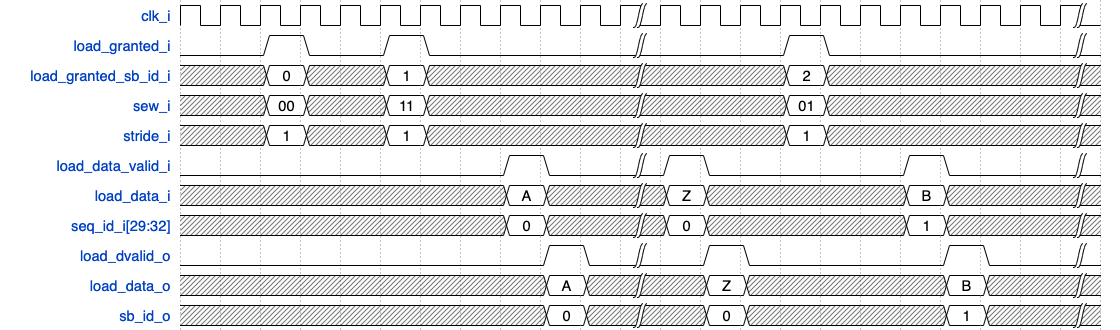
\includegraphics[scale = 0.35]{Chapter_2/img/lmu-time.png}
    \caption{Timing Diagram unit-strided load for the LMU}
    \label{lmu-time}
\end{figure}

In Figure \ref{lmu-time} it is possible to see an example for a unit-strided load. This is a simple load, and its behaviour will be discussed in the following section.

\subsubsection{Strided Load}
In this case all the valid elements are separated by a constant stride. If the stride is equal to 1, then is called unit-stride.\\

In Figure \ref{lmu-strided} there is a simple example to understand how the LMU works in this case.\\
The parameters (defined in the seq\+id\+i) are defining the elements to consider.
\begin{figure}[H]
    \centering
    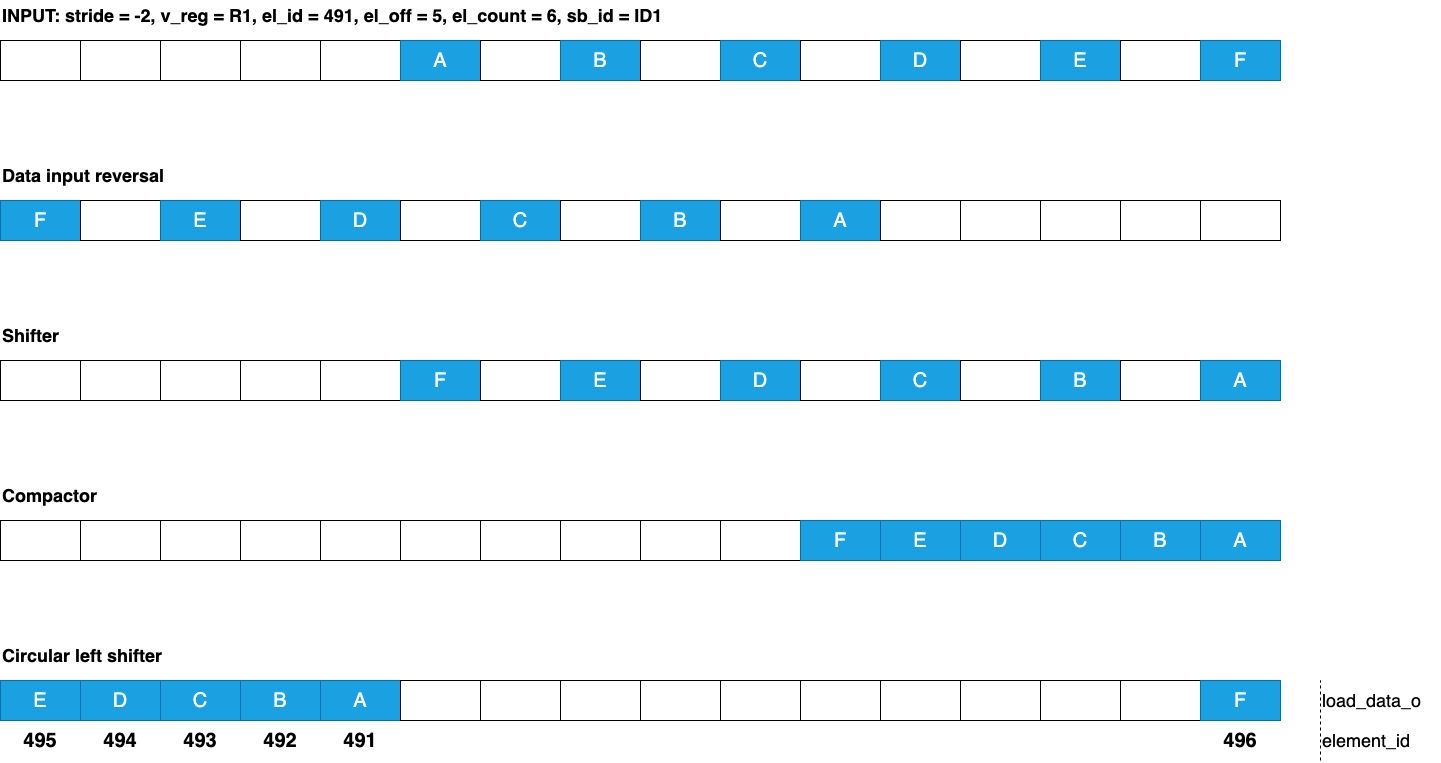
\includegraphics[scale = 0.25]{Chapter_2/img/lmu-strided.png}
    \caption{Strided load handled by the LMU}
    \label{lmu-strided}
\end{figure}

\subsubsection{Indexed Load}
It is also possible to load values in an indexed way. This means only one element at time is sent, and so the number of valid elements needs to be = 1.\\

In Figure \ref{lmu-indexed} it is possible to see an example for a simple indexed load.

\begin{figure}[H]
    \centering
    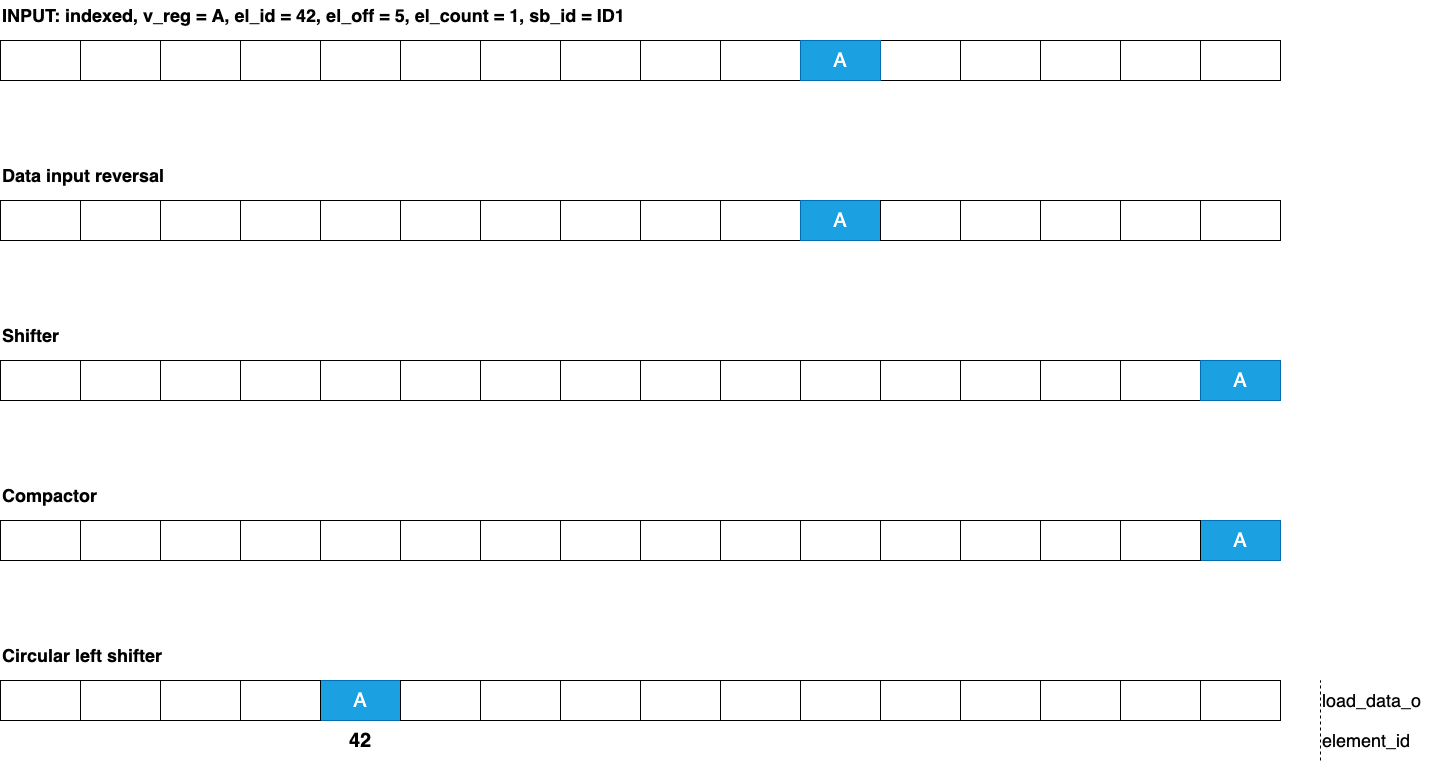
\includegraphics[scale = 0.25]{Chapter_2/img/lmu-indexed.png}
    \caption{Indexed load handled by the LMU}
    \label{lmu-indexed}
\end{figure}

\subsubsection{Masked Load}
All the load operations can be masked. This does not change the number of valid elements, but at the end of the process they not will be sent.\\


In Figure \ref{lmu-masked-stride} it is possible to see an example for the simple strided-load used before, but this time, with a mask.

\begin{figure}[H]
    \centering
    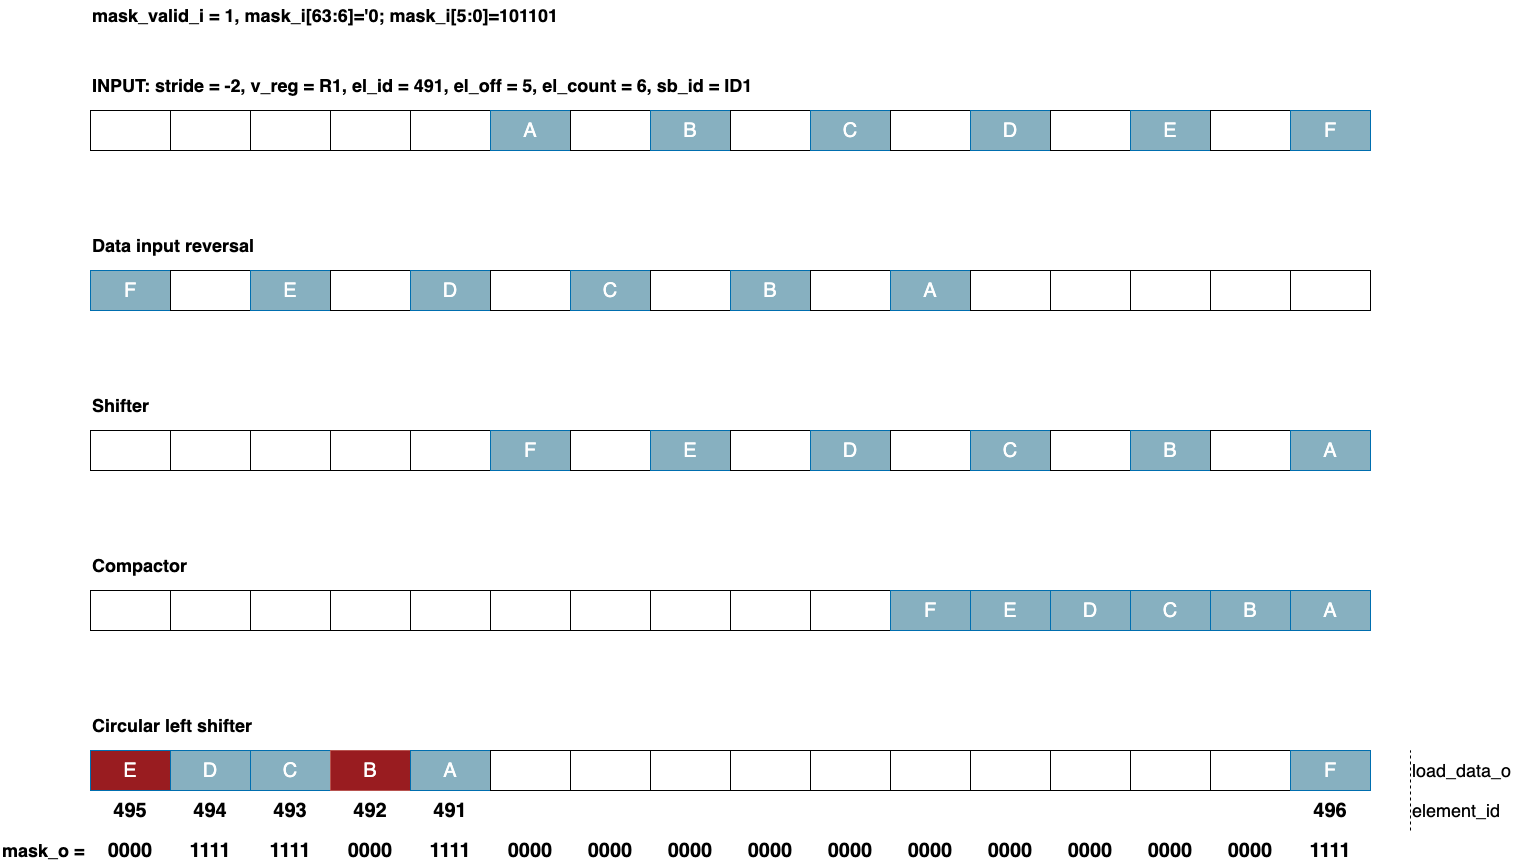
\includegraphics[scale = 0.25]{Chapter_2/img/lmu-masked-strided.png}
    \caption{Strided load, with mask, handled by the LMU}
    \label{lmu-masked-stride}
\end{figure}

\subsection{Load Buffer}
The second submodule that is mainly in charge of a load operation is the Load Buffer.\\
It is in charge of writing the data sent by Avispado to the Vector Register File. The data can be from different instructions inflight, and the Buffer will always try to optimize and group the data to write.\\

The LMU receives full cache lines of 512 bits from Avispado and forwards them to the corresponding Load Buffer for each lane (64 bits max per lane), depending on the seq\+id\+i. The postion of the data into the LB will be determined by the element ID.\\

Up to 2 loads can arrive, but they can come out-of-order, although the implementation will be parametrized to accept N loads in flight.
\subsubsection{Interface}
%%tables????

\subsubsection{Structure}
There is a Load Buffer of each lane and there are 3 layers to buffer the elements. The layers are divided by the concept of Element Group. In fact the elements cannot be disposed in every combination, but every element, based on its element ID, has an exact location (based also on the sew).\\
%elements 64 e 32

In Figure there is an example for the disposition of the elements for 64 bit or 32 bit. It is also important to say the number of bit for each element group stays the same, this means the number of element depends on the sew.\\

The layers of the LB are composed mainly of 4 parts:
\begin{itemize}
    \item Elements: the elements in the buffer;
    
    \item Identifier: identifies the elements coming from the young or the old load;
    
    \item Valid: identifies if the elements are valid;
    
    \item Element Group: identifies the eg, it is assigned by considering the VRF structure.
\end{itemize}

\subsubsection{Retry}
There are cases in which 3 layers are not enough to store all the elements. Indeed it is possible that more elements have the same position and so also 4 element can cause a problem, if they try to fit.\\

This case is handled with a retry mechanism:\\
an element is discarded and a new request is made to Avispado, to  notify the retry.\\

Is important to understand the element to discard when there is a retry, if the new one or the old one.\\

There are 4 possible cases:
\begin{enumerate}
    \item if the incoming data is from the young load and the buffer only contains data from the same load, it will be discarded the data with the highest element group;
    
    \item if the incoming data is from the young load and the buffer contain data from both the oldest and youngest loads, it will discard the incoming data;
    
    \item if the incoming data is from the old load and the buffer only contains data from the same load, it will be discarded the data with the highest element group;
    
    \item if the incoming data is from the old load and the buffer contain data from both the oldest and youngest loads, it will discard the data inside the buffer, the one from the young load.
\end{enumerate}



\subsubsection{Flow}
In figure 
%schema flow
it is possible to see a simple scheme of the LB's behaviour.
%describe the flow

\section{Verification Plan}
To have a good approach with the verification of a design, it is important to define a Verification Plan.\\
There are a lot of ways to do it, and most of the times they can be automatized to better perform in long term support of them. In this specific case, the Verification Team was working along with the Design Team to produce better specifications and not only to test a completed design. This means the Verification Plan is done following the general rules to have a good value in future, but it is not entirely defined a priori.\\

It was defined before to create the UVM structure and led to the development of all the tools for the verification. \\
To define the approach to have also means to define the tools to use, in fact different of them were created:
\begin{itemize}
    \item \textbf{UVM}: is the structure described before, used to stimulate and test the DUT;
    
    \item \textbf{checkers}: are some really powerful statements used to define the constraints of the DUT's behaviour. They can be used in different approaches. Later on this chapter it will be discussed their use as Functional or Formal tools;
    
    \item \textbf{coverage}: is the driver of the plan. It says were to work, and were there are tests to do. 
    
\end{itemize}
\subsection{Test Plan}

\section{Functional Verification}

\section{Formal Verification}

